\documentclass[12pt,a4paper]{article}
%\usepackage[left=0.8in,right=0.8in,top=1in,bottom=1in]{geometry}

\usepackage[superscript,biblabel]{cite}
\usepackage[parfill]{parskip}
% \usepackage{microtype} \hyphenpenalty=750


\usepackage[pdftex]{graphicx}
\usepackage{epstopdf}
% \DeclareGraphicsRule{.tif}{png}{.png}{`convert #1 `dirname #1`/`basename #1 .tif`.png}
\usepackage[utf8]{inputenc}
\usepackage{booktabs}
\usepackage[english]{babel}
\usepackage{siunitx} 
\sisetup{%
    range-phrase=--,
    range-units=single
    }

\usepackage{gensymb}
\usepackage{eurosym}

\usepackage[colorlinks]{hyperref}
\usepackage{caption} \captionsetup{labelfont={sf,bf}, size=footnotesize}
\usepackage{afterpage}

% set format of document title
\usepackage{titling}
\pretitle{\begin{center}\Large\bfseries} \posttitle{\end{center}\vspace{1em}}
\preauthor{\begin{center}\large} \postauthor{\end{center}\vspace{1em}}
\predate{\begin{center}\large} \postdate{\end{center}\vspace{1em}}
\pretitle{\begin{center}\Large\bfseries} \posttitle{\end{center}\vspace{1em}}

% set formats of section headings
\usepackage[explicit]{titlesec}
\titleformat{\title}{\centering}{\thesection.}{0.5em}{\MakeUppercase{#1}}
\titleformat{\section}{\centering}{\thesection.}{0.5em}{\MakeUppercase{#1}}
% \titleformat{\section}{}{\thesection.}{0.5em}{\MakeUppercase{#1}}
%\titleformat{\subsection}[runin]{\slshape}{\thesubsection.}{0.5em}{#1. }
\titleformat{\subsection}{\slshape}{\thesubsection.}{0.5em}{#1 }
\titleformat{\subsubsection}[runin]{\slshape}{\thesubsubsection.}{0.5em}{#1. }
 
\usepackage[T1]{fontenc}
\usepackage[scaled=.90]{helvet} \renewcommand{\familydefault}{\sfdefault} \usepackage[helvet]{sfmath}

\sisetup{detect-all} % tell siunitx to detect font stuff
 
\setlength{\columnsep}{0.75cm} 

\graphicspath{{figures/}}

\providecommand{\figr}[1]{Fig.~\ref{fig:#1}}
\providecommand{\figlabel}[1]{\label{fig:#1}}
\providecommand{\tabl}[1]{Tab.~\ref{tab:#1}}
\providecommand{\tablabel}[1]{\label{tab:#1}}
\providecommand{\sectn}[1]{Sec.~\ref{sec:#1}}
\providecommand{\seclabel}[1]{\label{sec:#1}}

\providecommand{\inductor}[1]{L\textsubscript{#1}}
\providecommand{\capacitor}[1]{C\textsubscript{#1}}
\providecommand{\resistor}[1]{R\textsubscript{#1}}

\providecommand{\Ohm}{$\Omega$}

% \interfootnotelinepenalty=10000


\title{The Open Source Monkey Coffin Loudspeaker} \author{Matthias Brennwald} \date{\today}

\usepackage{etoolbox}
\makeatletter
\patchcmd{\@maketitle}{\vskip 2em}{\vspace*{-2cm}}{}{}
\makeatother


\begin{document}


\maketitle
\vfill


\begin{center}
  \makebox[\textwidth]{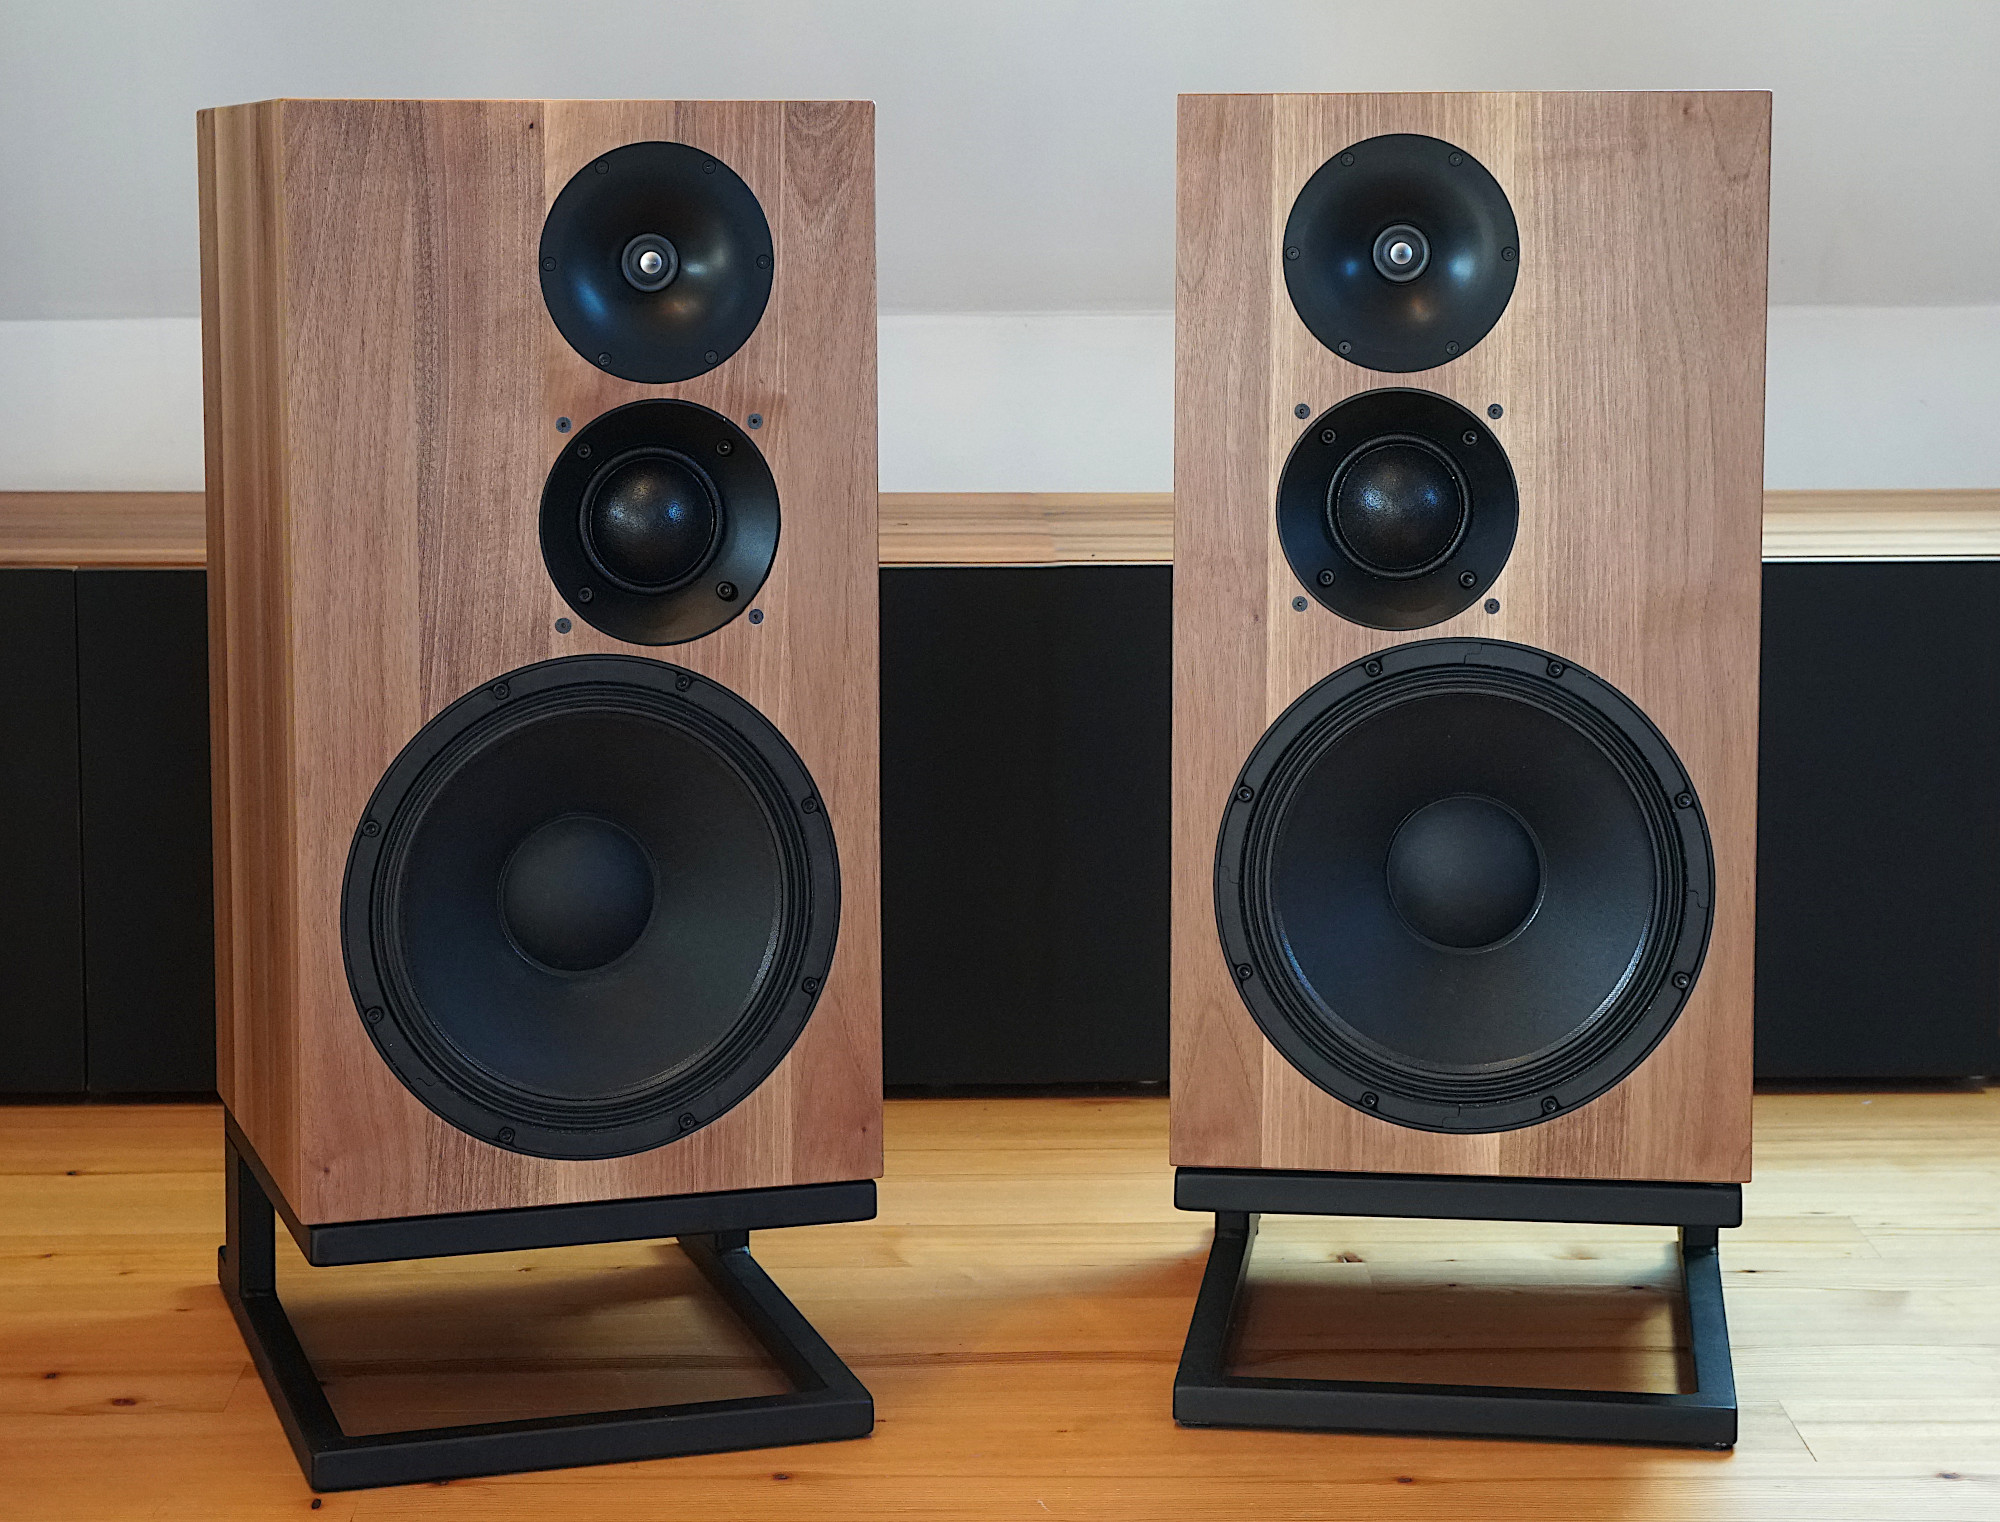
\includegraphics[width=\paperwidth]{osmc_photo.jpg}}
\end{center}

\thispagestyle{empty}

\clearpage

\vspace{0.2\textheight}

\section*{Important Notes and Disclaimers}
This document describes the design of the Open Source Monkey Coffin (OSMC) loudspeaker, which was developed in an ``open-source project''\cite{osmc_p1}. The aim of this project is to provide the OSMC design to DIYers for their own private purposes, for example to build a copy of the OSMC. Do not use the information developed in this project on a larger scale without written permission (for example by selling speakers based on the OSMC design or substantial parts of it).\par

The OSMC development was financially supported by diyAudio members LORDSANSUI, Paul Vancluysen, George Wright, KaffiMann, Charles Bueche, zimmer64, John Barbor, mbrennwa, and other anonymous members. Thank you!

\clearpage

\section{Overview}
The Open Source Monkey Coffin (OSMC) loudspeaker was developed by members of the diyAudio internet forum\cite{osmc_p1}. The motivation for developing this loudspeaker emerged from two diyAudio threads discussing the idea of ``open source'' loudspeaker designs\cite{osproj1_p1,osproj2_p1}. Once the types of loudspeakers that would appeal to many novice DIYers were identified, the design targets for the OSMC were defined as follows:

\begin{itemize}
\item The OSMC must be straight forward to make for DIY novices.
\item The box format should follow the ``large monitor'' format, sometimes also referred to as ``monkey coffin'' (hence the name). The internal volume should not be larger than \SIrange{60}{80}{L}. The enclosure must be a simple rectangular box which is easy enough to make on a kitchen table.
\item The OSMC should be ``amplifier friendly''. It should work well with small amplifiers like the popular Amp-Camp-Amp, tube amps, etc.
\item The OSMC should be a three way loudspeaker.
\item Keeping part costs low is not of paramount priority. If the right parts cost a lot of money and there are no cheaper equivalents, it's okay to use those parts in the design.
\end{itemize}

\clearpage


\section{System Design}

For ``amplifier friendliness'', the loudpseaker efficiency was targeted to \SI{92}{dB-SPL} at \SI{1}{m} and \SI{2.83}{V} input voltage, with a bass extension to 45 Hz (\SI{-3}{dB}). The impedance curve must not exhibit any sharp peaks or dips, and the OSMC should qualify as an ``\SI{8}{\Ohm} speaker''. It must be noted that, given the constraints of the box size, these targets could only be achieved if mechnical losses within the loudspeaker system were virtually zero, which is nearly impossible in real-world loudspeakers. While it is therefore not realistic to fully implement these design targets, these targets still provide useful guidelines for the design process.\par

The following is a brief summary of the design process, which is fully documented in the diyAudio thread.\cite{osmc_p1}The OSMC design was supported by the use of loudspeaker CAD tools (LEAP, Vituix CAD, Tolvan Edge). Measurement data were acquired using an RTX6001 USB audio analyser, MATAA software, and Earthworks M23 and iSEMcon EMX-7150 microphones. Data from measurements and simulations are available in the OSMC data repository\cite{osmc_datarepo}.


\subsection{Drivers}\seclabel{drivers}

High-quality drivers and parts should be chosen based on the technical specations required for the OSMC design. The look of the drivers has to be ``right'' for a HiFi system in a home environment (people may not want to build a speaker that looks unusual), but is second priority after the techincal specifications.

The woofer will determine the compromise between box size, bass-extension, and efficiency. 
The size of the woofer critically determines the efficiency of the loudspeaker, and a 12" woofer will just fit the targeted box size. After screening numerous woofers based on their specifications, Thielle-Small parameters, and tests of harmonic distortion the FaitalPro 12PR320 woofer was selected.\cite{osmc_p162,osmc_p236}

The midrange driver needs to keep up with the requirements of the sound pressure level (SPL) and impedance. The Volt VM752 dome driver will work very well from \SI{400}{Hz} up to about \SI{3}{kHz}. While there may be other midrange drivers that could be used, the VM752 was chosen due to the general interest for this driver and because some of the OSMC designers had good experience using this driver.

The tweeter also needs to keep up with the SPL and impedance requirements. Classical dome or ring radiator tweeters were preferred by the OSMC designers. Also, the use of a waveguide seems favourable in order to match the dispersion of the tweeter to the midrange, to reduce the effects of baffle diffraction, to increase the on-axis efficiency, and to reduce non-linear distortion of the tweeter. Tweeters with high directivity tend to minimize acoustic interference with the waveguide at wavelengths similar to the throat diameter, which helps to avoid large SPL wiggles at high frequencies\cite{ringradiators_in_waveguides}. Therefore, the Scan~Speak R2904/7000 ring radiator was chosen. The R2904/7000 also features high electrical impedance, high efficiency, and very low harmonic distortion. Most of the design work was done with a Visaton WG148 waveguide, which was modified to fit the R2904/7000.\cite{WG148mod} However, the final design uses a custom-made waveguide, which was designed specifically for use in the OSMC by diyAudio user augerpro\cite{augerproWGcircular}. The augerpro waveguide is acoustically almost identical to the WG148\cite{osmc_p881}, but is very easy to fit on the R2904/7000. It is available for purchase via group buy at diyAudio.\cite{augerpro_groupbuy}

\figr{impedance_curves_drivers} and \figr{SPL_curves_raw} show the impedance and the SPL response of the drivers mounted in the OSMC box. These data were used as the basis for electro-acoustical modelling of the crossover filters.

\begin{figure}[tbp]
	\centering
	% \vspace{-10ex}
	\includegraphics[width=0.7\textwidth]{impedance_curves_drivers.eps}
	\caption{Impedance curves of the drivers mounted in the OSMC box (magnitude and phase).}
	\figlabel{impedance_curves_drivers}
\end{figure}

\begin{figure}[tbp]
	\centering
	\vspace{-10ex}
	\includegraphics[width=0.7\textwidth]{SPL_curves_raw.eps}
	\caption{SPL response curves of the woofer (Faital 12PR320, top), midrange driver (Volt VM752, center) and tweeter (Scan Speak R2904/7000 with WG148 wave\-guide) mounted in the Monkey Coffin prototype box, measured at \SI{2.83}{Vrms} and \SI{1}{m} distance from the drivers, on axis and at $\pm$15\degree, $\pm$30\degree, $\pm$45\degree, $\pm$60\degree, $\pm$75\degree\ and $\pm$90\degree\ horizontal angles (the red curves were measured on the side where the tweeter and midrange drivers are closer to the baffle edge, the blue curves are from the other side; the woofer data is symmetric). Above \SI{300}{Hz}, the curves show the anechoic response as obtained from gated impulse-response measurements. The anechoic curves were extrapolated to lower frequencies by splicing them with modelled low-frequency curves (see text).}
	\figlabel{SPL_curves_raw}
\end{figure}

The SPL response curves were obtained from gated impulse-response measurements, which yielded the anechoic SPL response above \SI{300}{Hz}. Measurements were taken at horizontal angles from \SI{-90}{\degree} to \SI{+90}{\degree} at \SI{15}{\degree} steps. The low-frequency parts of each SPL curve were calculated from the Thielle-Small parameters of the drivers (using LEAP) and a diffraction model of the Monkey Coffin baffle (using Vituix CAD).\cite{osmc_p555} The anechoic part and the low-frequency part of each SPL curve were merged using a ``soft splice'' in the frequency range where both parts of the curve overlapped consistently\cite{osmc_p568}. Finally, the phase response (not shown in \figr{SPL_curves_raw}) was determined by calculating the minimum phase from each of the merged SPL curves. The drivers show smooth SPL response curves throughout their intended operating range. The on-axis on-axis response of the Volt VM752 midrange shows a dip at \SI{2.3}{kHz}. This dip disappears in the off-axis curves, which indicates that this is an uncritical diffraction artifact related to the driver/waveguide geometry rather than a problematic resonant effect.\par


\subsection{Baffle and Cabinet}

\figr{osmc_enclosure} shows the OSMC cabinet. The dimensions of the baffle are largely deteremined by the space required for the drivers. The tweeter and midrange are horizontally offset relative to the center in order to spread effects of diffraction at baffle edges over wide frequency band as much as possible.

\begin{figure}[tbp]
	\centering
	\includegraphics[width=\textwidth]{osmc_enclosure_20190823.pdf}
	\caption{Drawing of the OSMC enclosure. Notes: (1) the horizontal driver offsets are mirrored in the left and right speakers; (2) the rear must be removable for installation of the Volt VM752 driver; (3) the front needs to be \SI{20}{mm} thick to fit the Volt VM752 flange; (4) the speaker terminal hole shown here fits a Neutrik NL8MPR-BAG 8-pole Speakon terminal (adjust as suitable).}
	\figlabel{osmc_enclosure}
\end{figure}

The cabinet volume and the dimensions of the bass-reflex port were determined using simulations and measurements of the bass tuning. The goal was to obtain flat SPL response down to the cut-off frequency. In order to keep group delay low, the bass SPL curve was designed to roll off smoothly \figr{osmc_bass_tuning} shows the $2\pi$ free-field bass SPL response and the corresponding group delay. The SPL curve was determined using the microphone-in-box technique\cite{Small_inbox} for data up to \SI{110}{Hz}, which were spliced to a near-field measurement from \SI{90}{Hz} upwards. Note that this $2\pi$ SPL curve (solid line in \figr{osmc_bass_tuning}) assumes an infinite baffle and therefore does not show the baffle step as it occurs at the transition from the $4\pi$ radiation at low freqencies to $2\pi$ at higher frequencies. To estimate the true $4\pi$ SPL response of the woofer the OSMC box (dashed line in \figr{osmc_bass_tuning}), the OSMC baffle step was modelled using the Tolvan Edge simulator.

\begin{figure}[tb]
	\centering
	\includegraphics[width=0.6\textwidth]{osmc_bass_tuning.eps}
	\caption{Top: bass SPL response for \SI{2.83}{Vrms} drive voltage, at \SI{1}{m} (solid line: $2\pi$ response as measured using the microphone-in-box method\cite{Small_inbox}, dashed line: estimated $4\pi$ response taking into account the modelled baffle-step loss). Bottom: group delay determined from $2\pi$ SPL response. See also text).}
	\figlabel{osmc_bass_tuning}
\end{figure}


\subsection{Crossover filters}\seclabel{crossover_filters}

The crossover filters are implemented as passive circuits using steep filters in order to achieve small overlaps between the drivers in the crossover frequency bands, which reduces acoustic interferences between the drivers.

Full compensation for the baffle diffraction loss was designed into the crossover filters. The modelled curves of the diffraction loss were subtracted from the $2\pi$ SPL response curves of the raw drivers (see \sectn{drivers}). These SPL curves were used to design the filters to achieve a balanced $4\pi$ SPL response.\par

Two different filter types were considered during the prototyping process.\cite{osmc_p685} The first prototype uses elliptic filters, which are not very widely used in conventional loudspeaker designs. While the transfer functions of elliptic filters may exhibit some ripple near their cut-off range, they allow very steep slopes. The second prototype was designed with simpler and more conventional circuit topology using series inductors and parallel capacitors for the low-pass sections, and vice-versa for the the high-pass sections. Both prototypes were optimized for smooth and flat overall system SPL response, smooth dispersion and power response, and symmetric acoustic filter slopes near the cross-over points. The summed SPL curves in the filter simulations were virtually identical.

Both filter prototypes were implemented for testing in the OSMC prototype using a miniDSP digital signal processor. Acoustic measurement results with these DSP filters were similar for both filters, whereas the elliptic filters resulted in slightly more refined sound in listening tests\cite{osmc_p708}. The elliptic filters were therefore implemented as passive circuits and further optimized using acoustic measurements and listening tests. The schematic of the final cross-over filters is shown in \figr{osmc_EL_xover_schem}, with the part specifications in \tabl{OSMC_EL_xover_parts}.

\begin{figure}[p]
	\centering
	\includegraphics[width=\textwidth]{osmc_EL_xover_schem.pdf}
	\caption{OSMC cross-over filters (elliptic).}
	\figlabel{osmc_EL_xover_schem}
\end{figure}

\begin{table}[p]

\centering
\caption{List of parts in \figr{osmc_EL_xover_schem} (version 2019-08-23).}
\footnotesize
\tablabel{OSMC_EL_xover_parts}
\begin{tabular}{ccp{0.68\textwidth}} 
\toprule
Part & Value & Description\\ 
\midrule 
% \multicolumn{3}{c}{Woofer filter}\\
% \midrule

% woofer parts
\inductor{W1}	& \SI{6.8}{mH} / \SI{0.19}{\Ohm}	& Laminated iron core (e.g.~Mundorf BS180, Feron, I core, baked varnish)\\
\inductor{W2}	& \SI{1.8}{mH} / \SI{0.09}{\Ohm}	& Laminated iron core (e.g, Mundorf BS180, Feron, I core, baked varnish)\\
\inductor{W3}	& \SI{0.1}{mH} / \SI{0.23}{\Ohm}	& Air core (e.g.~Mundorf BL71, baked varnish)\\
\inductor{W4}	& \SI{15}{mH}  / \SI{1.12}{\Ohm}	& Iron core (e.g, Mundorf BH71, Ferrite, baked varnish)\\
\capacitor{W1}	& \SI{118}{\micro F}			& Parallel combination of \SI{100}{\micro F} bipolar electrolytic  (e.g.~Mundorf ECAP50) and \SI{18}{\micro F} MKP (e.g.~Mundorf MCAP250)\\
\capacitor{W2}	& \SI{33}{\micro F}			& Bipolar electrolytic (e.g.~Mundorf ECAP70)\\
\capacitor{W3}	& \SI{267}{\micro F}			& Parallel combination of \SI{220}{\micro F} and \SI{47}{\micro F} bipolar electrolytics (e.g.~Mundorf ECAP63 / ECAP50)\\
\resistor{W1}	& \SI{6.8}{\Ohm} / \SI{10}{W}		& MOX type (e.g.~Mundorf MR10)\\
\resistor{W2}	& \SI{5.6}{\Ohm} / \SI{10}{W}		& MOX type (e.g.~Mundorf MR10)\\

\midrule

% midrange parts
\inductor{M1}	& \SI{1.2}{mH} / \SI{0.44}{\Ohm}	& Air core (e.g.~Mundorf BL125, baked varnish)\\
\inductor{M2}	& \SI{0.33}{mH} / \SI{0.15}{\Ohm}	& Air core (e.g.~Mundorf BL100, baked varnish)\\
\inductor{M3}	& \SI{6.8}{mH} / \SI{0.46}{\Ohm}	& Iron core (e.g.~Mundorf BH100, Ferrite, baked varnish)\\
\inductor{M4}	& \SI{0.12}{mH} / \SI{0.15}{\Ohm}	& Air core (e.g.~Mundorf BL100, baked varnish)\\
\inductor{M5}	& \SI{2.7}{mH} / \SI{1.01}{\Ohm}	& Iron core (e.g.~Mundorf BP71, Ferrite, baked)\\
\capacitor{M1}	& \SI{33}{\micro F}			& MKP (e.g.~Mundorf MCAP250)\\
\capacitor{M2}	& \SI{267}{\micro F}			& Parallel combination of \SI{220}{\micro F} bipolar electrolytic (e.g., Mundorf ECAP63) and \SI{47}{\micro F} MKP (e.g.~Mundorf MCAP250)\\
% \capacitor{M3}	& \SI{6.8}{\micro F}			& MKP (e.g.~Mundorf MCAP250)\\
\capacitor{M3}	& \SI{5.6}{\micro F}			& MKP (e.g.~Mundorf MCAP250)\\
\capacitor{M4}	& \SI{4.7}{\micro F}			& MKP (e.g.~Mundorf MCAP250)\\
\capacitor{M5}	& \SI{68}{\micro F}			& Bipolar electrolytic (e.g.~Mundorf ECAP50)\\
\resistor{M1}	& \SI{2.7}{\Ohm} / \SI{10}{W}		& MOX or wire wound (non-inducitve) (e.g.~Mundorf MRES20)\\
\resistor{M2}	& \SI{5.6}{\Ohm} / \SI{10}{W}		& MOX or wire wound (non-inducitve) (e.g.~Mundorf MRES20)\\
\resistor{M3}	& \SI{8.2}{\Ohm} / \SI{10}{W}		& MOX or wire wound (e.g.~Mundorf MR10)\\
\resistor{M4}	& \SI{8.2}{\Ohm} / \SI{10}{W}		& MOX or wire wound (e.g.~Mundorf MR10)\\

\midrule

% tweeter parts
\inductor{T1}	& \SI{0.18}{mH} / \SI{0.38}{\Ohm}	& Air core (e.g.~Mundorf BL71, baked varnish)\\
\inductor{T2}	& \SI{0.47}{mH} / \SI{0.64}{\Ohm}	& Air core (e.g.~Mundorf BL71, baked varnish)\\
\capacitor{T1}	& \SI{4.7}{\micro F}			& MKP (e.g.~MCAP250)\\
\capacitor{T2}	& \SI{15}{\micro F}			& MKP (e.g.~MCAP250)\\
\capacitor{T3}	& \SI{100}{\micro F}			& Parallel combination of \SI{82}{\micro F} bipolar electrolytic and \SI{18}{\micro F} MKP (e.g.~Mundorf ECAP50-82 and MCAP250-18)\\
\capacitor{T4}	& \SI{100}{\micro F}			& Bipolar electrolytic (e.g.~Mundorf ECAP50)\\
\resistor{T1}	& \SI{3.9}{\Ohm} / \SI{10}{W}		& MOX or wire wound (non-inducitve) (e.g.~Mundorf MRES20)\\
\resistor{T2}	& \SI{1.0}{\Ohm} / \SI{10}{W}		& MOX or wire wound (non-inducitve) (e.g.~Mundorf MRES20)\\
\resistor{T3}	& \SI{4.7}{\Ohm} / \SI{10}{W}		& MOX type (e.g.~Mundorf MR10)\\
\bottomrule
\end{tabular}
\end{table}



\section{Construction}

\subsection{Estimated Costs}
The costs for a complete speaker are dominated by the drivers and the x-over parts. The costs for the cabinet depend a lot on the materials used. The estimated cost per speaker is as follows (not including taxes and shipping):

\begin{tabular}{lcp{0.3\textwidth}} 
\toprule
Part & Cost (\euro) & Remarks\\ 
\midrule 
Woofer (FaitalPRO 12PR320)	&	120	\\
Midrange (Volt VM752)		&	500 \\
Tweeter (Scan Speak R2904/7000)	&	250	\\
Tweeter waveguide (augerpro)	&	85	& diyAudio group buy\cite{augerpro_groupbuy} \\
X-over parts			&	300	& Parts as in \tabl{OSMC_EL_xover_parts} \\
Cabinet				&	approx.~100	& Basic MDF or plywood cabinet \\
Damping materials		&	approx.~50	& Basotect, sheeps wool \\
Bits and pieces			&	approx.~50 	& Bass reflex port, screws, wires, connectors, etc. \\
\midrule 
Total				&	approx.~1500 \\
\bottomrule
\end{tabular}


\subsection{Baffle and Cabinet}
The OSMC cabinet is a simple rectangular box and is straightforward to build (\figr{osmc_enclosure} and \figr{osmc_photos}). The rear wall should be removable to facilitate the rear mounting of the midrange driver. Internal braces reduce vibrations of the cabinet walls.\par

Any standing waves (modes) that develop in the enclosure need to be attenuated by suitable damping materials inside the enclosure. The mode along the vertical axis of the enclosure has a wavelength of $2 \times \SI{0.638}{m} = \SI{1.28}{m}$, which corresponds to \SI{269}{Hz}. This mode is attenuated using melamine foam absorbers (Basotect, Ewos ME50SK Pyramid) at the bottom and the top, and some sheeps wool the top, as shown in \figr{osmc_photos}. Any potential modes along the horizontal axes (left/right, rear/front) would exhibit considerably shorter wavelengths that correspond to frequencies of $\SI{450}{Hz}$ and higher, which are above the pass band of the woofer. These odes are therefore hardly excited and therefore do not require special attention. Also, the sound radiated from the woofer into the enclosure is reflected at the read wall. Another Basotect layer covering lower half of the rear wall is used to reduce this unwanted reflection. The remaining internal surfaces of the enclosure are covered with a thin layer of melamine foam only (use a large knive to remove the excess material as shown in \figr{osmc_photos}). There may also be other materials and arrangements of sound absorbers inside the enclosure that may lead to good results, and builders are encouraged to tweak the OSMC sound character in the low midrange and bass to their tastes. As a general rule, however, make sure not to obstruct the space between the woofer and the bass-reflex port.

\begin{figure}[tbp]
	\centering
	\includegraphics[height=0.55\textheight]{osmc_front.jpg}
	\hfill
	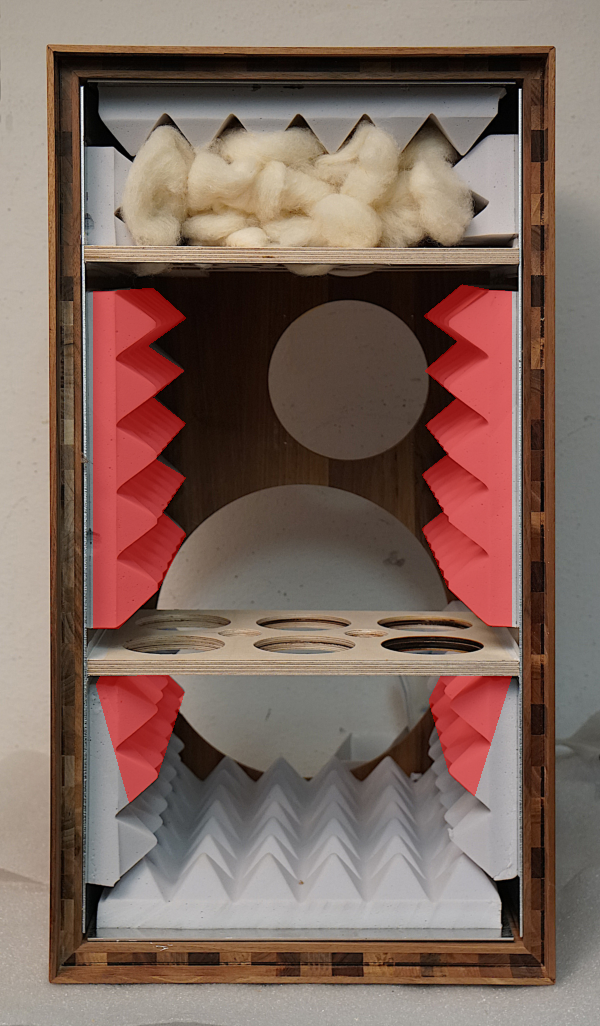
\includegraphics[height=0.55\textheight]{osmc_cabinet_open_damping.pdf}
	\caption{OSMC front and back with rear wall removed to show the bracing and damping. The red parts of the Basotect absorbers are removed using a large knive.}
	\figlabel{osmc_photos}
\end{figure}

The bass reflex port (type Monacor BR-100HP / Jantzen HP 900028) is cut to length and are then press-fit mounted in the rear wall. To ensure a tight seal between the rear baffle and the flange of the port, the flange may be wrapped with a few layers of tape. The recommended port length is approximately \SIrange{8}{9}{cm} long\cite{osmc_p918}, but slightly different port lengths (\SI{7}{cm} to \SI{11}{cm}) can be used to tweak the bass response. A longer port will cause a lower bass tuning with a softer roll off, whereas a shorter port will cause a higher bass tuning with a slight bass peak.

\subsection{Fitting the Tweeter Waveguide}
To mount the tweeter waveguide to the Scan Speak R2904 driver, the original faceplate needs to be removed from the tweeter by removing the three Torx screws. Note that the three empty screw holes that were used to fix the original faceplate to the tweeter would cause air leaks from the rear chamber, resulting in an undesired bass reflex tuning of the tweeter.\cite{scan_waveguide_bassreflex} The screw holes therefore need to be sealed with silicone or similar in order to maintain the desired tuning of the tweeter resonance.\cite{scan_waveguide_seal} The waveguide is fixed to the tweeter either using a clamp\cite{osmc_p1070} bolted to the rear of the waveguide (\figr{waveguide_sandwich}), or using a thin layer of silicone or similar glue.


\begin{figure}[tbp]
	\centering
	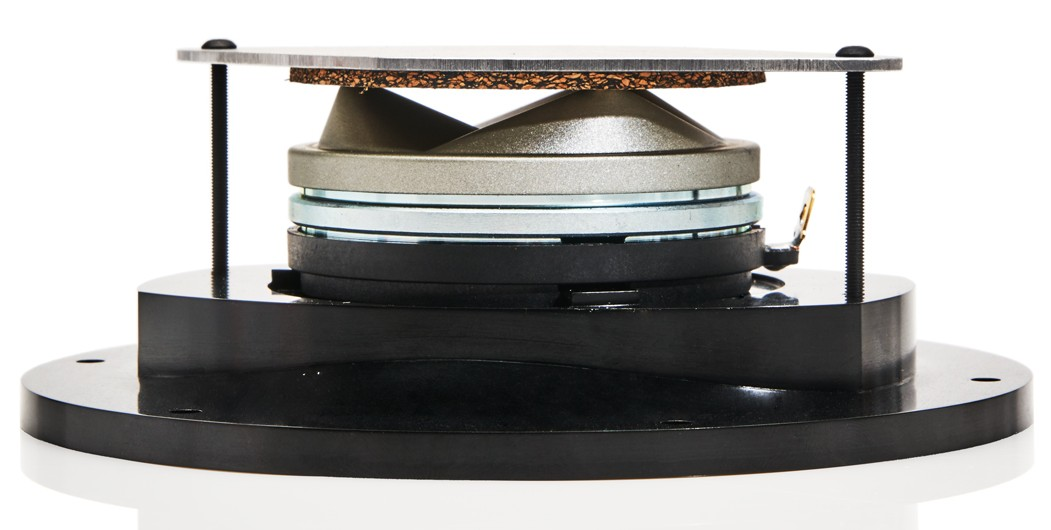
\includegraphics[width=0.8\textwidth]{waveguide_sandwich.jpg}
	\caption{Photo of the R2904 tweeter mounted on the waveguide using a clamp.}
	\figlabel{waveguide_sandwich}
\end{figure}

\subsection{Crossover Filters}
\figr{osmc_xover_construction} shows the construction of the x-over filters according to \figr{osmc_EL_xover_schem}. The parts are fixed to a base and connected to each other using flying leads. Given the size and complexity of the x-over circuits, it make sense to build the filters for the tweeter, midrange and woofer as separate modules, and to mount these modules in a separate box instead of in the OSMC cabinet. In order to minimize magnetic comupling and crosstalk between the different inductors, the inductors should be arranged perpendicular to each other and separated from each other as much as possible.\cite{osmc_p833}

Note that the manufacturers and type numbers of the parts suggested in \tabl{OSMC_EL_xover_parts} correspond to the parts used in the OSMC prototype. These are high quality parts and work well, but they may be substituted with other parts with the same specifications. It must be noted, however, that expensive boutique parts do not always yield better sound. For instance, the ``high-end'' MKP capacitors shown in \figr{osmc_xover_construction} resulted in bloated and euphonic sound, and were later replaced by other MKP capacitors.\cite{MKPtypes}

\begin{figure}[tbp]
	\centering
	\includegraphics[height=0.26\textheight]{xover_modules.jpg}
	\hfill
	\includegraphics[height=0.26\textheight]{xover_box.jpg}
	\caption{Construction of the crossover filter. Left: filter modules for the woofer, midrange, and tweeter. Right: complete crossover for one channel.}
	\figlabel{osmc_xover_construction}
\end{figure}


\section{System tests and performance}

\subsection{Electronic}
\figr{osmc_impedance_curve} shows the OSMC impedance vs.\ frequency. The impedance reaches its minimum value of \SI{4.8}{Ohm} at \SI{33}{Hz}, and ranges from \SI{5.5}{Ohm} to \SI{12.8}{Ohm} above \SI{45}{Hz}. There are no sharp variations in the impedance curve, which is also expressed in the rather flat curve of the impedance phase. The OSMC is therefore an easy load for the amplifier, even if the targeted ``\SI{8}{Ohm}'' rating\cite{osmc_p904} is valid only above \SI{100}{Hz} in a strict sense.

\begin{figure}[tbp]
	\centering
	\includegraphics[width=0.7\textwidth]{osmc_impedance_curve.eps}
	\caption{Measured electrical impedance (magnitude in blue, phase in red).}
	\figlabel{osmc_impedance_curve}
\end{figure}

\figr{osmc_filter_transfer} shows the OSMC filter transfer curves. The leakage in the stop bands of the elliptic filters is obvious for the midrange filter. However, the efficiency of the midrange driver in the respective frequency bands is very low (\figr{SPL_curves_raw}), and the attenuation in the stop bands is \SI{-25}{dB} or better. The filter leakage is therefore considered irrelevant.

\begin{figure}[tpb]
	\centering
	\includegraphics[width=0.7\textwidth]{osmc_filter_transfer.eps}
	% note: this shows the 2019-03-03 version of the filter, where the kink in the tweeter transfer curve is a bit stronger than it should be.
	\caption{Measured transfer curves of the crossover filters for the woofer (blue), midrange (black), and tweeter (red).}
	\figlabel{osmc_filter_transfer}
\end{figure}


\subsection{Acoustic}
\figr{osmc_step_response} shows the free-field OSMC step response with the typical 3-way sequence of the tweeter peak followed by the peaks of the midrange and the woofer. The transitions between the peaks are smooth, and no resonances or other time-domain issues are apparent.

\figr{osmc_SPL_response} shows the anechoic free-field ($4\pi$) on-axis SPL response. The part of the response curve above $\SI{330}{Hz}$ was determined from the anechoic part of the impulse response. The bass response of the OSMC system was determined from the $4\pi$ far-field woofer response (\figr{osmc_bass_tuning}) and the woofer x-over filter curve (\figr{osmc_filter_transfer}). The the bass \SI{-3}{dB} cut-off is at \SI{50}{Hz}, as targeted in the design goals. The efficiency is \SI{90}{dB-SPL} (\SI{1}{m}, \SI{2.83}{V}) in the bass range. As expected, this is slightly less than the design goal, which is based the theoretically achievable optimum for system zero losses. Overall, the SPL response is very linear and shows a slight trend of decreasing SPL at higher frequencies. This decrease is required to compensate the progressive beaming of the waveguides in order to achive the desired slope of the power response curve (see below). The small dip at \SI{2.2}{kHz} is a baffle-diffraction effect that is not apparent in the off-axis response.\par

\figr{osmc_polar} shows the SPL dispersion of the OSMC. Both the horizontal and vertical dispersion are well controlled and are generally very smooth. Beaming increases smoothly towards higher frequencies. The vertical dispersion shows a cancellation at the x-over between the midrange driver and the tweeter. However, due to the steep x-over filters, this artifact is limited to a rather narrow frequency band.\par

The in-room SPL curve of the OSMC in a generic room was estimated from the sound power radiated into the listening environment (power response, \figr{osmc_powerresponse}). The power response was calculated by summing the polar SPL reponse data over a virtual sphere around the loudspeaker.\cite{tylka,mat_lspr} Systematic listening studies in typical home environments showed that listeners preferred a smooth and linear in-room SPL response curve, and they perceived the sound as balanced if the in-room response showed a decreasing trend towards higher frequencies.\cite{osmc_p915} These features are nicely demonstrated in the OSMC power response. Note that the OSMC loudspeaker approaches constant directivity behaviour. The on-axis response curve therefore needs to show a similar decreasing trend as the power response curve in order to achieve balanced sound.


\begin{figure}[p]
	\centering
	\includegraphics[width=0.7\textwidth]{osmc_step_response.eps}
	\caption{Step response at \SI{1}{m} (anechoic part).}
	\figlabel{osmc_step_response}
\end{figure}

\begin{figure}[p]
	\centering
	\includegraphics[width=0.7\textwidth]{osmc_SPL_response.eps}
	\caption{SPL response at \SI{1}{m} (on axis, free field / $4\pi$, see text).}
	\figlabel{osmc_SPL_response}
\end{figure}

\begin{figure}[p]
	\centering
	\includegraphics[width=0.8\textwidth]{osmc_polar_horizontal.eps}\\
	\includegraphics[width=0.8\textwidth]{osmc_polar_vertical.eps}
	\caption{SPL dispersion (top: horizontal dispersion, bottom: vertical dispersion).}
	\figlabel{osmc_polar}
\end{figure}

\begin{figure}[p]
	\centering
	\includegraphics[width=0.7\textwidth]{osmc_powerresponse.eps}
	\caption{Power response (see text).}
	\figlabel{osmc_powerresponse}
\end{figure}

\begin{figure}[p]
	\centering
	\includegraphics[width=0.7\textwidth]{osmc_CSD_diagram.eps}
	\caption{Cumulative spectral decay diagram.}
	\figlabel{osmc_CSD_diagram}
\end{figure}


\clearpage


\subsection{Listening impressions}
The OSMC was designed for accurate music playback in a home environment with ``amplifier friendliness'' in mind. Listening tests were therefore conducted with a \SI{11}{W} tube amplifier (triode push pull design) and a \SI{25}{W} solid state amplifier (FirstWatt F5 class-A). These amplifiers had no problems driving the OSMC to ``party levels'', which confirms the ``amplifier friendliness'' of the OSMC.\par

The overall sound is balanced and coherent, with tight, articulate and well controlled bass. As an inevitable physical consequence of the ``amplifier friendliness'', however, the bass is not as deep as with some other similar sized ``HiFi'' loudspeakers that need to be driven by powerful amplifiers. The OSMC sounds highly transparent and dynamic, both at low and high playback levels. This lack of compression allows good resolution of low-level details even with complex or loud music. The waveguides result in a large proportion of direct sound at the listener position, resulting in precise rendering of the musical scene with less impact of the reverberant sound of the room.

\clearpage

% list of references
\bibliographystyle{unsrt}
\bibliography{osmc_refs}


\end{document}
